% Document
\documentclass{article}

% Packages
\usepackage[utf8]{inputenc}                                                             % input encoding
\usepackage[T1]{fontenc}                                                                % font encoding
\usepackage[ngerman]{babel}                                                             % for German
\usepackage[left=2cm, right=2cm, top=2.5cm,bottom=2.5cm]{geometry}                      % for page size
\usepackage{natbib}                                                                     % for bibliography
\usepackage{graphicx}                                                                   % for images
\usepackage[font=normal,labelfont=bf,textfont=rm,position=bottom,skip=10pt]{caption}    % for captions
\usepackage{amsmath}                                                                    % for formulas
\usepackage{float}                                                                      % for images at right position
\usepackage[autostyle=true,german=quotes]{csquotes}                                     % for proper quotes
\usepackage{siunitx}                                             

% for MATLAB-codes
\usepackage{comment}
\usepackage{bm}
\usepackage{hyperref}
\usepackage{pdfpages} %fuer einfuegen von PDFs (Aufgabenstellung)
% for block comments

\newcommand{\geodaten}[1]{\underline{#1}}     % Vektor als Matrix

% Document start
\begin{document}
\section{}
Kepler Elements to perifocal Frame: 
\begin{equation*}
	\bm{r_f} = \left(\begin{matrix}
		a \cdot \left(\cos E-e\right) \\
		a \cdot \sqrt{1-e^2} \cdot \sin E \\
		0
	\end{matrix}\right)
\end{equation*}
\begin{equation*}
	\bm{\dot{r}_f} = \frac{n_a}{1-a \cdot \cos E}\left(\begin{matrix}
		-\sin E \\
		\sqrt{1-e^2} \cos E \\
		0
	\end{matrix}\right)
\end{equation*}
To ecef
\begin{equation*}
	\bm{r_e} = R_3(-\Omega) R_1(-I) R_3(-\omega) \bm{r_f}
\end{equation*}
\begin{equation*}
	\bm{\dot{r}_e} = R_3(-\Omega) R_1(-I) R_3(-\omega) \bm{\dot{r}_f}
\end{equation*}
\\
\\
Frage: ist folgende Gleichung gültig in ecef?
\begin{equation}\label{eq1}
	d \left(\begin{matrix}
		\bm{r_e} \\
		\bm{\dot{r}_e}
	\end{matrix}\right) = \left(\begin{matrix}
	\bm{\dot{r}_e} \\
	-\frac{GM}{r^3} \cdot \bm{r_e}
\end{matrix}\right) + \left(\begin{matrix}
\bm{0} \\
\bm{f_e}
\end{matrix}\right)
\end{equation}
\\
Da $\bm{r_e}$ vorhanden ist, kann man Länge, Breite und Höhe berechnen, mit den kriegt man die Atmosphäre Dichte $\rho$. Dann kann man aus $\rho$ und $\bm{\dot{r}_e}$ die Atmosphärische Widerstand $\bm{f_e}$ berechnen mit \autoref{eq2} Formen(Angenommen, die Geschwindigkeit von Atmosphäre ist 0):
\begin{equation}\label{eq2}
	\bm{f_e} = -\frac{1}{2} \cdot C_d \cdot \rho \cdot \frac{A}{m} \cdot \bm{\dot{r}_e} \cdot |\bm{\dot{r}_e}|
\end{equation}
\\
Wenn \autoref{eq1} gültig ist, kann man die Koordinaten in ecef mit Runge-Kutta (ode45 Funktion in matlab) integrieren. Am Ende transformiert man die Koordinaten zurück in Kepler Element.

\section{}
\begin{figure}[H]
	\centering
	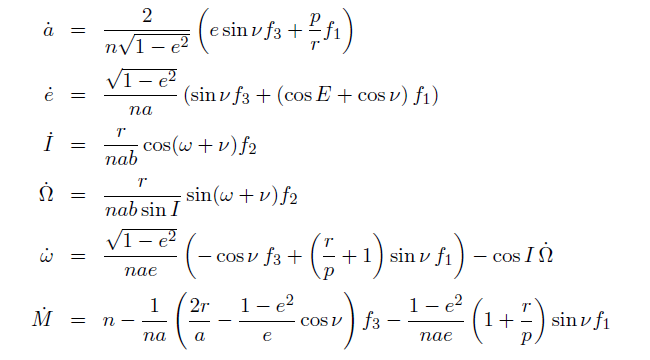
\includegraphics[width=0.8\textwidth]{LPE.png} 
	\caption{} \label{fig:1}
\end{figure}
Vereinfachung ($e=0$):
\begin{figure}[H]
	\centering
	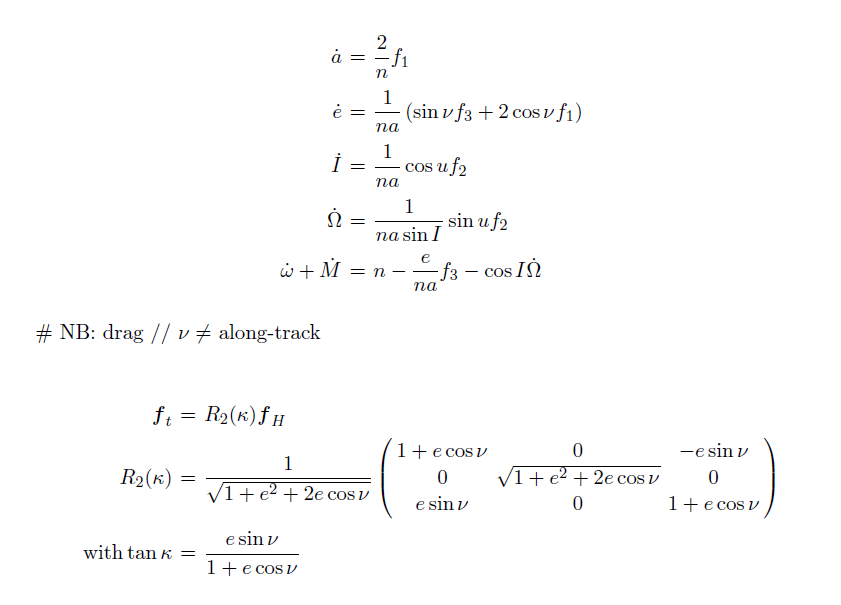
\includegraphics[width=0.8\textwidth]{LPE2.png} 
	\caption{} \label{fig:2}
\end{figure}
Das heißt, man kann direkt auf Kepler Element integrieren, aber $f$ muss man zuerst in t-frame transformieren. 
\end{document}



